\section{Versuchsaufbau und Messmethoden} 

    \subsection{Versuchsaufbau}
    \label{sec:Aufbau}

        \noindent Der prinzipielle Aufbau des Experimentes ist in \autoref{fig:schema_aufbau} dargestellt. Die Probe befindet sich mitten in einer Spule in einem möglichst homogenen Magnetfeld, welches senkrecht zu der Spule steht.
        Mit dem \enquote{Sender} können Pulse an die Spule gegebn werden, sodass hochfrequente Magnetfelder in der Spule entstehen. Wird die Magnetisierung in der Spule angeregt, so präzediert diese in der 
        $x$-$y$-Ebene und in der Spule wird durch das sich ändernde Magnetfeld eine Spannung induziert. Durch Relaxationsprozesse kehrt die Magnetisierung wieder in die Gleichgewichtslage zurück, dies wird 
        \enquote{freier Induktionszerfall} (FID) genannt. Die Spannung, welche durch den FID in der Spule entsteht, wird mit dem Empfänger gemessen. 

        \begin{figure}[H]
            \centering
            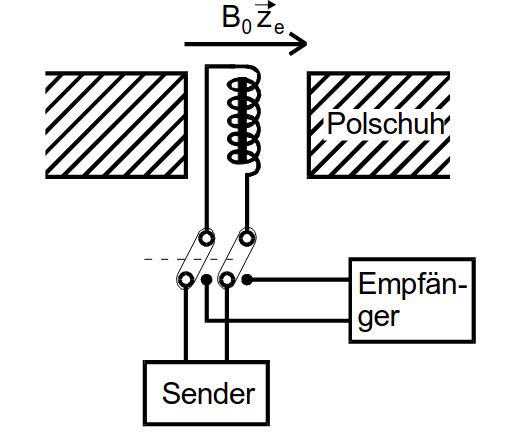
\includegraphics[width=0.3\textwidth]{latex/images/schema_aufbau.png}
            \caption{Der schematische Aufbau des Versuchs. \cite{finke}}
            \label{fig:schema_aufbau}
        \end{figure}

        \noindent In \autoref{fig:blockschaltbild} ist das Blockschaltbild eines NMR-Spektrometers zu sehen, wobei jedoch der Magnet, der das homogene Magnetfeld erzeugt, nicht eingezeichnet ist. Durch dieses Magnetfeld 
        spalten sich die Kernspin-Niveaus auf und eine Magnetisierung tritt auf. Die Spule ist, wie im obigen Bild um die Probe gelegen und wird zur Anregung und zur Messung genutzt. \\
        Das aufgenommene Signal der Spule geht nach einer Verstärkung in einen Splitter, genauso wie die hochfrequente (HF) Spannung für die Pulse. Diese werden dann so in einen Mischer gegeben, sodass sich 
        eine Spannung proportional zum Spin-Echo-Signal und dem Kosinuswinkel zwischen Referenz- und Probenspannung und eine hochfrequente Komponente einer Frequenz von etwa $2\omega_\text{L}$ ergeben. 
        In einen zweiten Mischer wird die Signalspannung aus dem anderen Splitterausgang mit der um $\SI{90}{\degree}$ verschobenen HF-Spannung gemischt. Hier ergibt sich als einziger Unterschied eine 
        Propotionalität zum Sinuswinkel. Die HF Anteile der Spannungen werden mithilfe eines Tiefpasses herausgefiltert. Dieses Verfahren entspricht der Quadraturdetektion. \\ 
        Die Signale werden dann vom Computer aufgenommen oder am Oszilloskop angezeigt. 
        Die Pulse werden mithilfe der Pulskarte, dem Frequenzgenerator, Schalter und Verstärker konfiguriert.

        \begin{figure}[H]
            \centering
            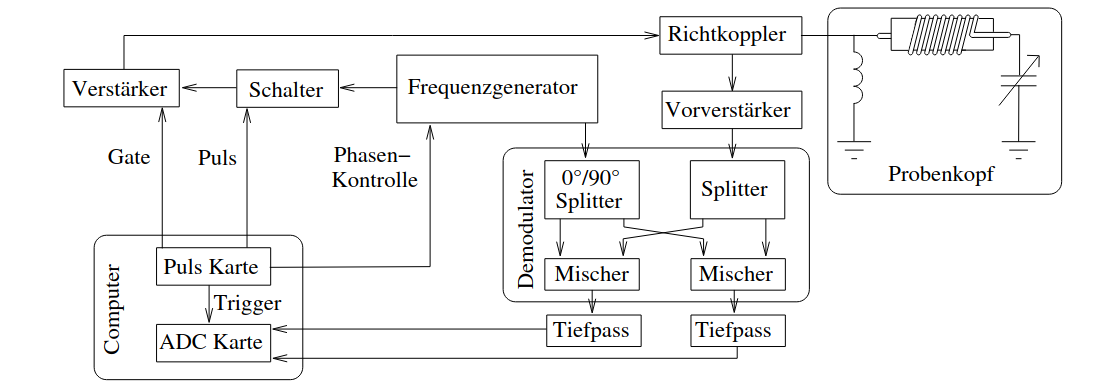
\includegraphics[width=\textwidth]{latex/images/blockschaltbild_nmr.png}
            \caption{Blockschaltbild eines NMR-Spektrometers. Der Magnet, in dem sich die Probe befindet, ist nicht dargestellt. \cite{grundlagen}}
            \label{fig:blockschaltbild}
        \end{figure}

        \noindent Damit der Empfangsverstärker bei den $\SI{90}{\degree}$- und $\SI{180}{\degree}$- Pulsen nicht übersteuert und zur Minimierung von Rauschen trennt der Richtkoppler Eingangs- und Ausgangssignal. 
        Er wird oft durch eine Diodenbrücke dargestellt, die erst ab $\SI{0.6}{\volt}$ eine Leitfähigkeit besitzt. So kann das Ausgangssignal einfach auf den Empfangsverstärker, da das Signal zu gering ist. 
        Die Pulse haben eine deutlich höhere Spannung, sodass diese durch die Diodenbrücke nur ein wenig verkleinert werden. Die Rauschspannung des Sendeverstärkers wird so aber nicht an den Empfangsverstärker 
        gegeben. 

        \noindent Der Versuch in schon vollständig aufgebaut, es muss lediglich eine Justage durchgeführt werden. 

    \subsection{Messmethoden}
    \label{sec:Messmethoden}

    \subsubsection{Inversion Recovery}

        Mit einem $\SI{180}{\degree}$ Puls wird $M_z$ invertiert und durch einen $\SI{90}{\degree}$-Puls nach der Zeit $t$ 
        in messbare Quermagnetisierung umgewandelt. Die messbare FID-Amplitude ist ein Maß für die relaxierte $z$-Magnetisierung, es gilt 
        \begin{equation*}
            M_z(t) = M_\infty \left(1 - 2e^{-\frac{t}{T_1}}\right)\, .
        \end{equation*}
        Die Bedingung $M_z(0) = M_\infty$ ist wegen Inhomogenitäten des anregenden Magnetfeldes nicht erfüllt. \\
        Das Verfahren ist graphisch noch in \autoref{fig:T_1} dargestellt. 

        \begin{figure}%
            \centering%
            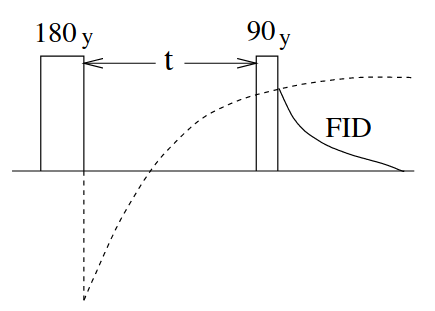
\includegraphics[width=0.3\textwidth]{latex/images/t_1_messung.png}%
            \caption{Das Inversion Recovery Verfahren zur Messung der Spin-Gitter Relaxationszeit $T_1$. \cite{grundlagen}}%
            \label{fig:T_1}%
        \end{figure}%

    \subsubsection{Spin-Echo}

        \noindent Hier wird die Magnetisierung erst mit einem $\SI{90}{\degree}$ Puls in die $y'$-Richtung gelegt, wie es in \autoref{fig:hahn} Teil \(a\) gezeigt ist. Dann präzedieren die Spins 
        um die $z$-Achse. Da die einzelnen Spins alle leicht unterschiedliche Magnetfelder sehen, kommen sie bald aus der Phase, welches in \(b\) zu sehen ist. Die Spins sind soweit auseinandergelaufen, 
        dass kein Induktionssignal mehr erzeugt wird. Zum Zeitpunkt $\tau$ nach dem ersten Puls wird ein $\SI{180}{\degree}$ geschalten, sodass die Spins alle einzeln invertiert werden \(c\). 
        Die Spins laufen jetzt wieder zusammen, dass bei $2 \tau$ die Spins wieder alle in Phase liegen und ein Induktionssignal gemessen werden kann, wie es in \(d\) zu sehen ist.  

        \begin{figure}
            \centering
            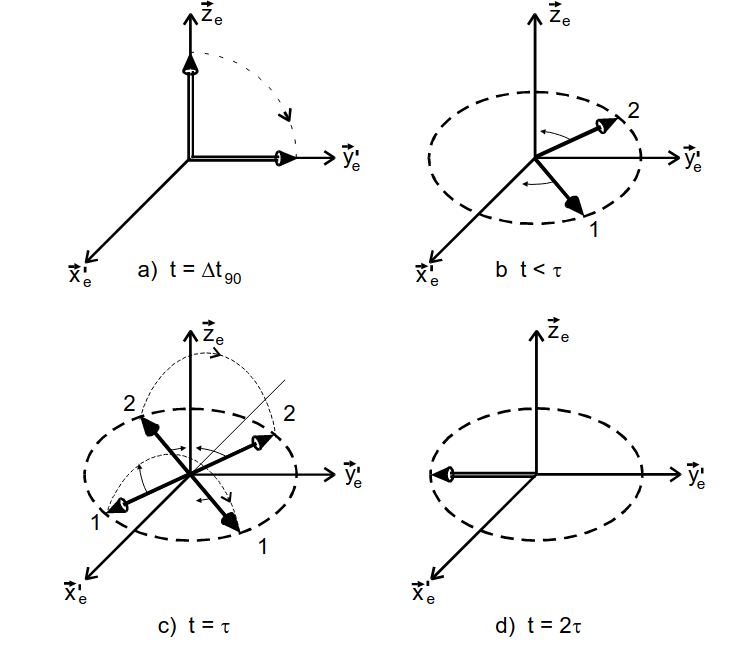
\includegraphics[width=0.8\textwidth]{latex/images/Hahn_echo.png}
            \caption{Zeitlicher Verlauf der Spin-Echo Methode. \cite{finke}}
            \label{fig:hahn}
        \end{figure}

        \noindent Neben den reversiblen Dephasierungsprozesse gibt es noch irreversible, welche auf der Wechselwirkung der Spins mit seiner Umgebung beruht. Die irreversiblen Dephasierungsprozesse 
        treten vermehrt mit größerem $\tau$ auf, sodass der Zusammenhang 
        \begin{equation}
            M_y(t) = M_0 \cdot \exp(-\frac{t}{T_2})
            \label{eqn:expT_2}
        \end{equation}
        aufgestellt werden kann. 
        
        \noindent Da immer gewartet werden muss, bis die Magnetisierung komplett relaxiert ist, bevor eine neue Messung mit einem anderen $\tau$ gestartet werden kann, wurde diese Methodik verbessert. 
        In der \textbf{Carr-Purcell} Methode wird nach dem ersten $\SI{90}{\degree}$-Puls eine Menge $\SI{180}{\degree}$-Pulse in einem Abstand von $2\tau$ geschalten. Dies ist in \autoref{fig:carr_purcell}
        dargestellt. 

        \begin{figure}
            \centering
            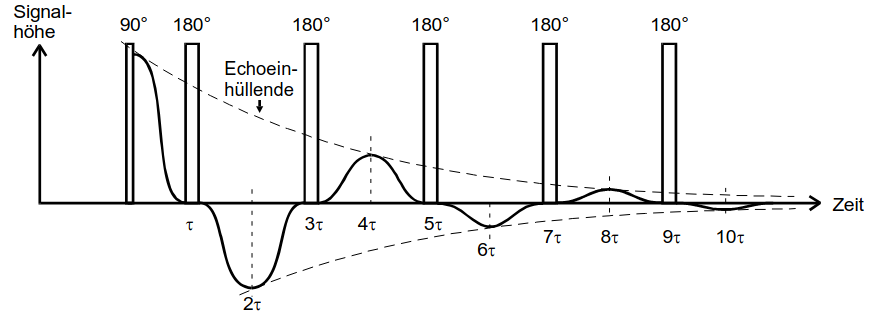
\includegraphics[width=\textwidth]{latex/images/Carr_Purcell.png}
            \caption{Die Pulsfolge der Carr-Purcell-Methode. \cite{finke}}
            \label{fig:carr_purcell}
        \end{figure}

        \noindent Die Spins werden also mit den wiederholten Pulsen wieder zu den Zeitpunkten $2 n \tau$, $n\in \symbb{N}$ fokussiert. Die Amplitude der Echos sinkt aufgrund der irreversiblen Dephasierungsprozesse. 
        Jedoch funktioniert die erneute Fokussierung nur, wenn der Puls genau zu dem Zeitpunkt kommt, an dem die Spins in Phase sind. Dies ist sehr schwer zu ermöglichen im experimentellen Aufbau. 
        Daher wird in der \textbf{Meiboom-Gill} Methode die HF Schwingungen in den $\SI{180}{\degree}$-Pulsen um $\SI{90}{\degree}$ in der Phase gegenüber dem $\SI{90}{\degree}$-Puls verschoben. 
        Damit werden die Spins nach dem ersten $\SI{180}{\degree}$-Puls nur noch um die $y'$-Richtung geklappt. Damit wird bei einer Fehljustierung bei jedem zweiten Puls der Fehler korrigiert. Also kann 
        jeder zweite Peak, welche alle ein positives Vorzeichen haben, genutzt werden, um eine Funktion der Art \eqref{eqn:expT_2} daran zu fitten und so $T_2$ zu ermitteln.
        
    \subsubsection{Diffusionsmessung}

        \noindent Aufgrund der Inhomogenität des Feldes wird auf das bestimmte $T_2$ die Relaxation $T_2^{\text{inhom}}$ aufaddiert, damit die effektive Abfallzeit $T_2^{\text{eff}}$ ermittelt werden kann. 
        Bei einem inhomogenen Feldgradienten kann die Diffusionskonstante $D$ ermittelt werden, da sich nun bei dem bekannten Feldgradienten $G$ eine Bewegung aus der Brownschen Molekularbewegung messbar eine andere Lamorfrequenz ergibt. 
        Es ergibt sich ein exponentieller Zusammenhang 
        \begin{equation*}
            A ( 2 \tau ) = \exp(-\frac{2}{3} D \gamma^2 G2 \tau^3)
        \end{equation*}
        für das erste Echo. Hierbei ist $\gamma$ das gyromagnetische Verhältnis. 
        Wird nun der Abstand $\tau$ zwischen dem $\SI{90}{\degree}$ und $\SI{180}{\degree}$-Puls erhöht kann die Funktion 
        \begin{equation*}
            M_y (t) = M_0 \exp\left(- \frac{2 \tau}{T_2}\right)\exp\left(- \frac{D \gamma^2 G^2 2 \tau^3}{3}\right)
        \end{equation*}
        an die Messwerte gefittet werden, solange der Zusammenhang 
        \begin{equation*}
            T_2^3 \gg \frac{3}{2 D \gamma^2 G^2}
        \end{equation*}
        gilt. 


\section{Durchführung}
\label{sec:durchführung}

    \noindent Zu Beginn wird das nach NMR-Spektromenter, welches nach Abschnitt \ref{sec:Aufbau} aufgebaut wurde, justiert. Anschließend wird die $T_1$- Relaxationszeit gemessen, da diese für die Messung von $T_2$ bekannt 
    sein sollte. Somit wird danach die Relaxationszeit $T_2$ gemessen.  Abschließend wird die Diffusionsmessung durchgeführt. Zur Illustration der Pulse und deren Abstände ist in \autoref{fig:schema_puls} eine Darstellung
    derer. 

    \begin{figure}[H]
        \centering
        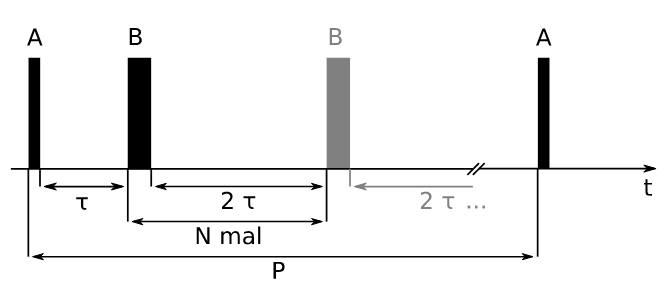
\includegraphics[width=0.4\textwidth]{latex/images/schema_puls.png}
        \caption{Schmematische Darstellung des Pulsprogrammes. \cite{V49}}
        \label{fig:schema_puls}
    \end{figure}

    \subsection{Justage}

        \noindent Zur Justage des NMR-Spektroskometer wird Wasser mit Kupfersulfat benutzt, da es eine geringe Relaxationszeit hat. Es werden die Startparameter eingestellt: 
        \begin{itemize}
            \item Frequenz $F = \SI{21.7}{\mega\hertz}$
            \item Pulslänge $A = \SI{2}{\micro\second}$
            \item Anzahl der B-Pulse $N = \num{0}$ 
            \item Periode $P = \SI{0.5}{\second}$ 
            \item Shims $x = \num{-1.0}$, $y = \num{-5.0}$, $z = \num{3.7}$, $z^2 = \num{-2.4}$
        \end{itemize}
        Anschließend wird die Frequenz genauer eingestellt. Da die Detektion relativ zur Lamorfrequenz erfolgt, sollte bei einer richtig eingestellten Frequenz keine Oszillation zu sehen sein. 
        Danach wird die Phase so eingestellt, dass der Realteil den Großteil des Signals trägt und der Imaginärteil minimal wird. Jetzt werden die Shims so verändert, dass der auf dem Oszilloskop 
        sichtbare FID möglichst lange geht und auch noch nach $\SI{2}{\milli\second}$ gut erkennbar ist. Es wird also die Feldhomogenität des Gradienten maximiert. \\
        Es werden die Pulszeiten für einen $\SI{90}{\degree}$ und $\SI{180}{\degree}$ Puls ermittelt. Dabei sollte zwischen den Zeiten ein Faktor 2 liegen, der $\SI{90}{\degree}$-Puls soll den 
        FID maximieren und der $\SI{180}{\degree}$-Puls soll den FID minimieren. \\
        Für die Untersuchung der Temperaturabhängigkeit wird noch die Temperatur in der Spule mit einem Thermoelement gemessen. 
        
    \subsection{$T_1$-Messung}

        \noindent Es wird die Pulslänge A auf die des $\SI{180}{\degree}$-Puls gestellt und die B-Pulslänge auf die des $\SI{90}{\degree}$-Puls. Die Anzahl des B-Pulses beträgt $N = 1$. Die Periode 
        wird auf $ P = \SI{10}{\second}$ gestellt, aber für $\tau > \SI{1}{\second}$ wird $P$ mindestens auf $\tau + \SI{10}{\second}$ gestellt.\\ 
        Es wird die Amplitude des FID nach dem B-Puls gemessen, mit Variablem $\tau$. Das kürzeste $\tau$ soll dabei so sein, dass noch keine Relaxation stattfindet, und das Längste so, dass die Magnetisierung 
        vollständig relaxiert ist. Dies entspricht einer Messung nach der Inversion Recovery Methode.

    \subsection{$T_2$-Messung}

        \noindent Nun wird einmal die Meiboom-Gill Messmethode angewendet. Dafür wird zuerst der A-Puls auf den $\SI{90}{\degree}$-Puls gestellt und der B-Puls auf die $\SI{180}{\degree}$-Pulslänge. Der 
        B-Puls soll $N= \num{100}$ mal wiederholt werden. Die Periode soll auf mindestens $3 T_1$ gestellt werden, damit die Magnetisierung vollständig relaxiert ist, bevor eine neue Pulsfolge beginnt. 
        Der Pulsabstand $\tau$ wird so gewählt, dass das Maximum des $\num{100}$ter Echos ungefähr $\frac{1}{3}$ des ersten Echomaximums beträgt. Von der Antwort des Systems auf eine solche Pulsfolge 
        wird mithilfe des Oszilloskops ein Bild gespeichert und die Daten der Peaks entnommen. \\ 
        Es wird der Knopf \enquote{MG} auf \enquote{off} gestellt und wieder ein Bild gespeichert. Dieses Messverfahren entspricht der Carr-Purcell-Messmethode. \\
        Für die Untersuchung der Temperaturabhängigkeit wird noch die Temperatur in der Spule mit einem Thermoelement gemessen.

    \subsection{Diffusionsmessung}

        \noindent Es wird der Feldgradient maximiert, in dem nur die $z$-Komponente auf ihren positiven maximalen Wert gestellt wird. Anschließend wird der A-Puls auf die $\SI{90}{\degree}$ Länge gestellt, 
        der B-Puls auf die $\SI{180}{\degree}$ Länge. Der B-Puls soll $N=1$ mal wiederholt werden, die Periode bleibt bei $3 T_1$. Es wird nun $\tau$ variiert, beginnend bei $\SI{100}{\micro\metre}$ 
        bis schließlich das Echo im Rauschen veschwindet. Für ein ausgewähltes kleines $\tau$ wird das Signal von Real- und Imaginärteil am Oszilloskop gespeichert. \\
        Für die Untersuchung der Temperaturabhängigkeit wird noch die Temperatur in der Spule mit einem Thermoelement gemessen.